% ============================================================================
% LITERATURE REVIEW - ADDITIONS AND EXPANSIONS
% ============================================================================

\subsection{Signal Generation}
\Ac{EIS} requires the generation of a small AC excitation signal, either voltage or current, to probe the \ac{DUT}. Generating or measuring voltage is simpler as most modern electronics are voltage mode rather than current mode. On the other hand, generating a small current signal is difficult to do accurately and requires circuits such as the improved Howland current pump \cite{ImprovedHowlandCurrent2020}. While measuring a current signal also has some complexity, it is significantly easier than generation and thus the method commonly used in \ac{EIS} systems.

Voltage-based signal generation can be done using dedicated impedance analyser chips such as the AD5933 or custom solutions using microcontroller-based \acp{DAC}. The AD5933 offers integrated frequency sweeps and impedance measurement. However, it has some clear drawbacks, such as a DC offset, lack of direct voltage measurement and minimum impedance of $1 k\Omega$.

Direct measurement of the true voltage across the device under test ensures all sources of non-ideal behaviour (parasitic resistances, stray capacitance, drift, and environmental changes) are accounted for, providing accurate data for impedance calculation. Accurate voltage monitoring is vital because small changes can significantly affect calculated impedance, particularly in low-voltage biosensing circuits. In contrast, a DAC and ADC solution implemented on a microcontroller allows for precise control of excitation signals, flexible signal processing, and easier integration with multiplexing and user interface subsystems.

\subsubsection{Bipolar Signals and DC Bias}
Biosensing requires a bipolar signal with no DC component to avoid charge accumulation at the electrode–electrolyte interface. Over time, a DC bias establishes a net electrochemical potential that drives unwanted redox reactions and alters the interfacial chemistry of the biosensor. These parasitic reactions change the impedance characteristics of the electrode, obscuring the dielectric and charge transfer properties that \ac{EIS} measurements aim to quantify. Ensuring a bipolar excitation centred around a stable reference prevents these effects and maintains measurement integrity.

\subsubsection{Anti-Aliasing Filters}
When generating a sinusoidal signal using a \ac{DAC}, the output is not a smooth analogue waveform, but rather a series of discrete voltage steps. These steps introduce high-frequency components and harmonics that are not present in the original signal. If these unwanted frequencies are not removed, they can interfere with downstream analogue circuitry or be misinterpreted during subsequent analog-to-digital conversion, a phenomenon known as aliasing. To prevent this, an anti-aliasing filter (AA filter), typically a \ac{LPF}, is placed after the DAC output to remove high-frequency content and smooth out the signal.

The dynamic range of a \ac{DAC}, expressed in decibels, determines the smallest signal it can produce above its noise floor and is given by Equation \ref{eq:dac_range_lit}\cite{gaddyDYNAMICPERFORMANCETESTING}:
\begin{equation}
    \text{Dynamic Range} = 6.02n + 1.76 
    \label{eq:dac_range_lit}
\end{equation}
with $n$ being the number of bits of resolution. The anti-aliasing filter must attenuate high-frequency components sufficiently so that any aliased content falls below the DAC's noise floor, whilst maintaining a flat passband response at the desired signal bandwidth to avoid distorting the amplitude or phase of the intended output.

For systems that generate signals across a wide frequency range, a fixed-frequency AA filter becomes unsuitable, as a single cutoff frequency cannot accommodate both low and high signal frequencies without either excessive attenuation or inadequate filtering. Variable AA filters address this by allowing the cutoff frequency to be adjusted dynamically. Many such filters require changing resistor values to set the cutoff frequency, which is impractical when rapid frequency changes are needed. Clock-tunable filters, which adjust their cutoff frequency based on an external clock signal, offer a more flexible solution for applications requiring wide frequency sweeps.

\subsection{Voltage Measurement}
Accurate voltage measurement across the \ac{DUT} is essential for impedance calculation. Some impedance analyser designs attempt to infer voltage across the sample by using the known characteristics of the applied signal \cite{buscagliaSimpleZLowCostPortable2023}. However, this approach fails to account for non-ideal behaviours such as parasitic resistances, stray capacitance, drift, and environmental changes. Direct measurement of the voltage ensures that all these variations are captured, leading to more reliable impedance calculations, particularly in low-voltage biosensing applications where even small errors can significantly impact results.

It is essential to measure the voltage directly across the biosensor itself, rather than measuring the applied signal only in reference to a fixed potential. This ensures that dynamic and non-ideal behaviours at the sensor–electrolyte interface are accurately reflected in the measurement.

\subsubsection{Differential Amplifiers vs Instrumentation Amplifiers}
Two common circuits are used to perform differential voltage measurements: differential op-amps and instrumentation amplifiers. Differential op-amps are simple and cost-effective for basic differential measurements, but they are susceptible to common-mode noise and offset errors \cite{technologyWhatAreDrawbacks2024}. They also have relatively low input impedance, which can load the signal source and affect test results \cite{technologyWhatAreDrawbacks2024}. 

Instrumentation amplifiers, on the other hand, are specifically designed for high-precision differential measurement and provide superior common-mode rejection, high input impedance, and excellent accuracy even when the input signals are small or operating in a noisy environment \cite{InstrumentationAmplifierOperational}. This makes instrumentation amplifiers particularly suitable for biosensing applications where the signals to be measured can be very small, and minimising interference is critical.

\subsubsection{Signal Amplification and ADC Range Utilisation}
It is important to amplify the measured voltage to fully utilise the linear range of the \ac{ADC}, which enhances both sensitivity and resolution. By maximising the voltage swing within the \ac{ADC}'s input range, the system can discriminate smaller changes in sensor response, thus allowing for better detection of low-concentration analytes. However, amplification introduces trade-offs related to gain-bandwidth product, which limits the usable bandwidth of the amplifier at higher gains. Multi-stage amplification can mitigate this limitation by distributing gain across several stages, allowing higher overall gain whilst maintaining adequate bandwidth across the measurement frequency range.

\subsection{Current Measurement}
Accurate current measurement is essential for determining the impedance of the \ac{DUT}. Two primary approaches exist: shunt resistor-based measurement and transimpedance amplifier-based measurement.

\subsubsection{Shunt Resistor vs Transimpedance Amplifier}
The most basic method of measuring current involves placing a small, known precision resistor (shunt resistor) in series with the current path and measuring the voltage drop across it. Using Ohm's Law, the current can then be calculated. This approach is cheap and easy to implement, but has severe drawbacks. The voltage drop across the resistor directly reduces the magnitude of the applied perturbation to the \ac{DUT}, thereby impacting the measurements. For biosensing, where signal levels are already low, even small drops or error sources can significantly affect sensitivity.

A \ac{TIA}, on the other hand, converts the input current to a proportional output voltage without introducing a significant voltage drop across the \ac{DUT}. The TIA leverages the properties of op-amps, where the inverting and non-inverting inputs are driven to the same potential, and the input bias currents are negligible. By connecting the \ac{DUT} to the inverting input (held at a virtual ground reference) and placing a feedback resistor between the output and inverting input, the current from the sensor flows entirely through the feedback resistor, producing an output voltage proportional to the input current. This configuration maintains a low-impedance path for the current whilst ensuring high input impedance, preventing the TIA from loading the \ac{DUT}.

\subsubsection{Variable Gain for Wide Dynamic Range}
In biosensing applications with a fixed voltage perturbation, the current can vary dramatically depending on the impedance of the \ac{DUT}—from nanoamperes at high impedance (low analyte concentration) to milliamperes at low impedance (high analyte concentration). A fixed-gain amplifier is impractical across this wide dynamic range, as it would either saturate at high currents or provide insufficient resolution at low currents. Variable gain amplification, achieved through switchable feedback resistors in the TIA or through \acp{PGA} in subsequent stages, allows the system to adapt to the current magnitude, ensuring that the output voltage remains within the optimal range for the \ac{ADC} whilst maximising measurement resolution.

% ============================================================================
% DESIGN SECTION - REVISED VERSIONS
% ============================================================================

\subsection{Excitation}\label{subsec:design_excitation}
The easiest way of producing a controlled voltage signal is using a \ac{DAC}. Both dedicated \acp{DAC} and \acp{DAC} built into \acp{MCU} were possible options.

To avoid establishing a DC bias at the electrode–electrolyte interface, the generated excitation must be centred around a stable reference potential. This can be achieved by shifting the DAC output to be biased around ground using a level-shifting op-amp circuit. However, this also requires providing all analogue circuitry with a negative supply rail. Rather, this project makes use of a buffered virtual ground reference at 1.65V (3.3V/2) and uses this as the midpoint for all the analogue circuitry. This approach ensures that no DC bias is applied to the \ac{DUT} whilst negating the need for negative supply rails.

The anti-aliasing filter must provide sufficient attenuation at the Nyquist frequency ($f_s/2$) to ensure that any aliased content falls below the DAC's noise floor. For the 12-bit \ac{DAC} found in the STM32F303K8, Equation \ref{eq:dac_range} gives a dynamic range of 74dB. 

\begin{equation}
    \text{Dynamic Range}=6.02n + 1.76 
    \label{eq:dac_range}
\end{equation}

At the same time, the filter's passband must remain flat at the desired signal bandwidth to avoid distorting the amplitude or phase of the intended output. Due to these requirements, a fixed frequency AA filter is unsuitable when generating a wide range of frequencies from 1Hz--100kHz.

Many variable AA filter ICs exist, however many require changing a resistor value to set the cutoff frequency, which would be impractical when many frequencies are needed. Ultimately the LTC1069 proved to be the only viable option, providing an 8th order lowpass filter that approximates a raised cosine response (with $\alpha=1$). Importantly it has a cutoff frequency of up to 120kHz (200kHz when using $\pm5V$ supply rails) set by an external clock and a linear phase response \cite{LTC10697CS8PBF}. The clock-tunable nature of the LTC1069 is ideal for this project, allowing easy adjustments through the use of a timer on the STM.

To maximise the voltage resolution and minimise noise, the full linear range of the DAC is utilised when generating the signal. This requires that the DAC output signal is attenuated from 3Vpp to the desired 10mVpp using an inverting op-amp. From Equation \ref{eq:inv_opamp_gain} $R_{f}=1k\Omega$ and $R_{in}=300k\Omega$ can be calculated as suitable values.

\begin{equation}
    A_v = \frac{V_{out}}{V_{in}} = -\frac{R_f}{R_{in}}
    \label{eq:inv_opamp_gain}
\end{equation}

\begin{figure}[]
    \centering
    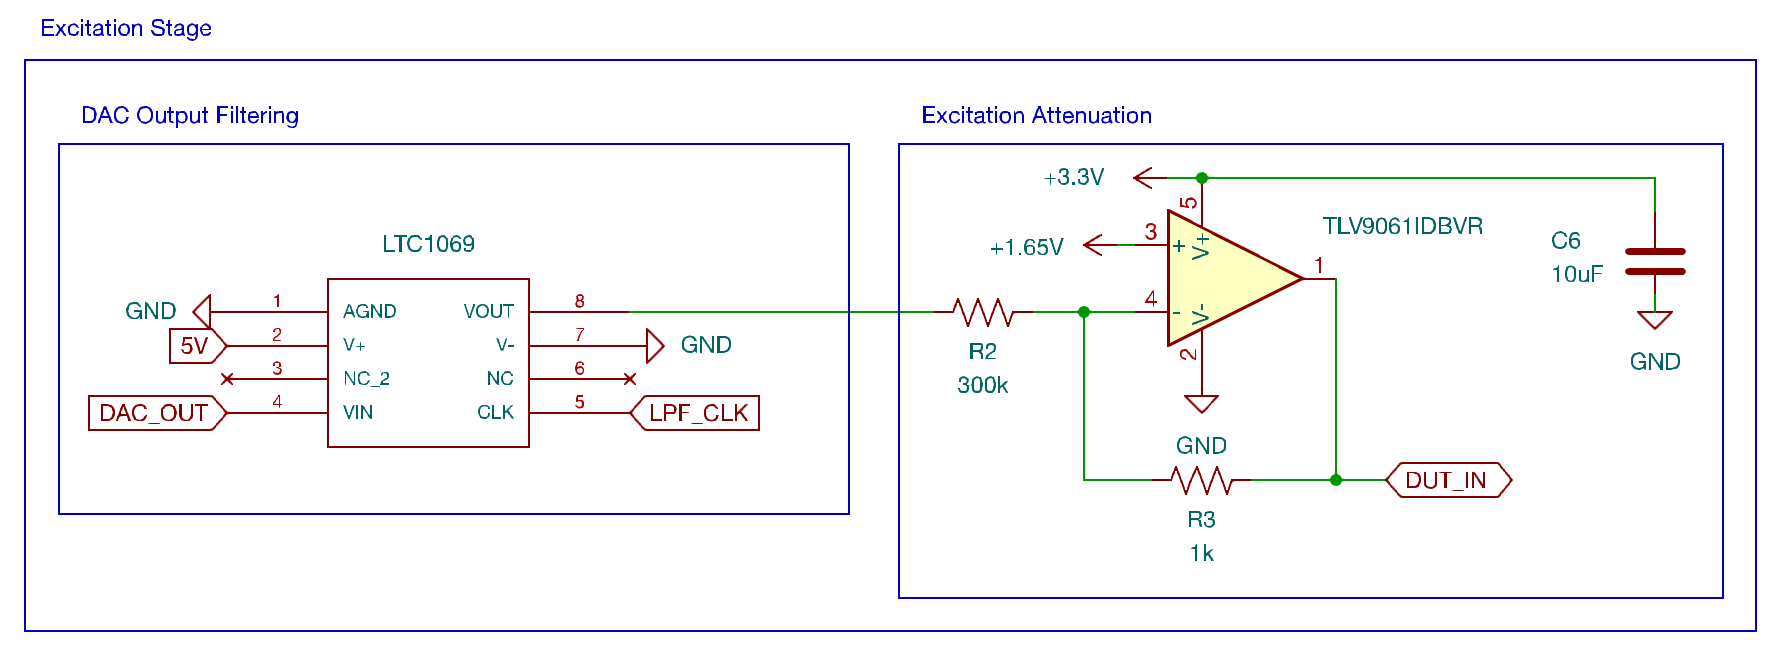
\includegraphics[width=\textwidth]{ExcitationSchem.png}
    \caption{Complete Excitation Stage Circuit}
    \label{fig:excitation_stage_circuit}
\end{figure}

\subsection{Voltage Measurement}
The INA331 instrumentation amplifier was selected for the first stage of voltage measurement due to its combination of low offset voltage, high common-mode rejection and low input bias current. The INA331 features a typical offset voltage of 250 µV, which represents the inherent DC error between the input terminals when no differential signal is applied. It directly adds to the measured voltage, creating a systematic DC error that must be considered in calibration. The low input bias current of 0.5pA avoids loading the DUT and influencing the current measurements. The device provides an internal gain of 5 V/V, configurable to higher gains through external resistors according to the relationship $G = 5 + 5\times \frac{R_2}{R_1}$. Choosing $R_1=1k\Omega$ and $R_2=2k\Omega$ results in a gain of 15V/V. 

\Ac{GBW} represents the -3dB bandwidth of an op-amp at unity gain. The -3dB bandwidth of the op-amp can then be calculated for a specific gain using Equation \ref{eq:GBW} where $A_{noise}$ represents the noise gain calculated in Equation \ref{eq:noise_gain}. The use of noise gain accounts for the non-ideal feedback effects and circuit imperfections \cite{fiore53GainBandwidthProduct2018}.

\begin{equation}
    f_c = \frac{GBW}{A_{noise}}
    \label{eq:GBW}
\end{equation}
\begin{equation}
    A_{noise} = 1 + \frac{R_f}{R_{in}}
    \label{eq:noise_gain}
\end{equation}

The gain and phase shift at any frequency can then be calculated based on the cutoff frequency using equations \ref{eq:mag_rollof} and \ref{eq:phase_shift} respectively \cite{oljacaOperationalAmplifierGain2010}. With $\omega=2\pi f$ and $\omega_0=2\pi f_c$.

\begin{equation}
    |H(j\omega)|_{dB} = 20\log\frac{1}{\sqrt{1+\frac{\omega^2}{w_0^2}}}
    \label{eq:mag_rollof}
\end{equation}
\begin{equation}
    \varphi(\omega) = -\tan^{-1}(\frac{\omega}{\omega_0})
    \label{eq:phase_shift}
\end{equation}

While equations \ref{eq:GBW} and \ref{eq:noise_gain} are not applicable to instrumentation amplifiers due to their three op-amp design, the bandwidth can be estimated from the datasheet to be 2.3MHz (as seen in Figure \ref{fig:ina_bw}) at the chosen gain. Using equations \ref{eq:mag_rollof} and \ref{eq:phase_shift}, the gain reduction and phase shift at 100kHz can be estimated as -0.004dB and -2.49\textdegree\ respectively. 

\begin{figure}[H]
    \centering
    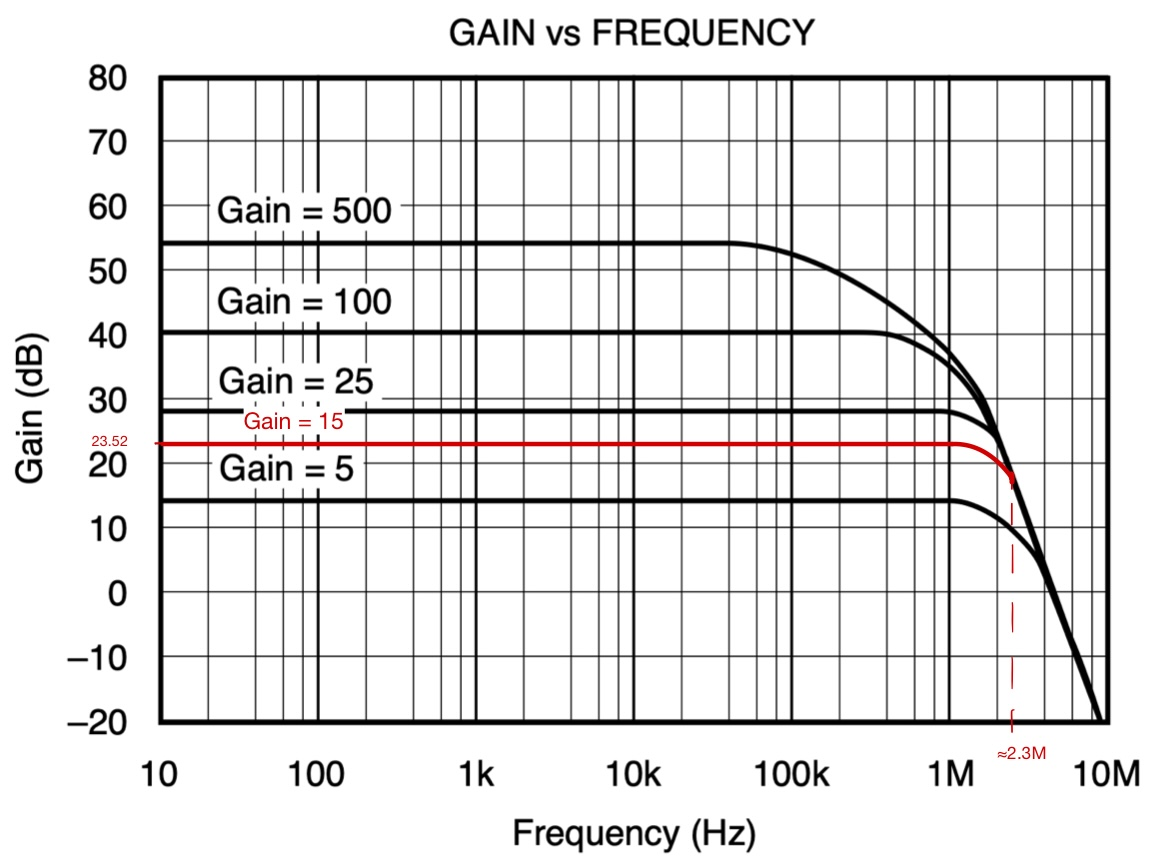
\includegraphics[width=0.5\textwidth]{INA_BW.jpeg}
    \caption{INA331 Bandwidth vs Gain adapted from \cite{INA331}}
    \label{fig:ina_bw}
\end{figure}

Using a single stage of amplification to amplify the signal from 10mVpp back to 3Vpp would introduce significant phase shifts and gain reductions at higher test frequencies due to \ac{GBW} limitations. This is alleviated by using a two-stage amplification design. The second amplification stage uses a TLV9061 op-amp in an inverting gain configuration. With a GBW of 10MHz and gain of $A_v=-20$ ($A_{noise}=21$) the expected bandwidth is 476.2kHz (Equation \ref{eq:GBW}). From equations \ref{eq:mag_rollof} and \ref{eq:phase_shift} an expected -0.094dB gain reduction and -11.86\textdegree\ phase shift is calculated at 100kHz. 

While the first stage still needs to be accounted for during calibration due to its very flat and linear response, the second stage does not need to be calibrated for as an identical gain stage will be used for the current measurement, ensuring that any gain reductions and phase shifts are cancelled out during impedance calculation.

The final circuit for voltage measurement can be seen in Figure \ref{fig:vmeas_stage_circuit}.

\begin{figure}[H]
    \centering
    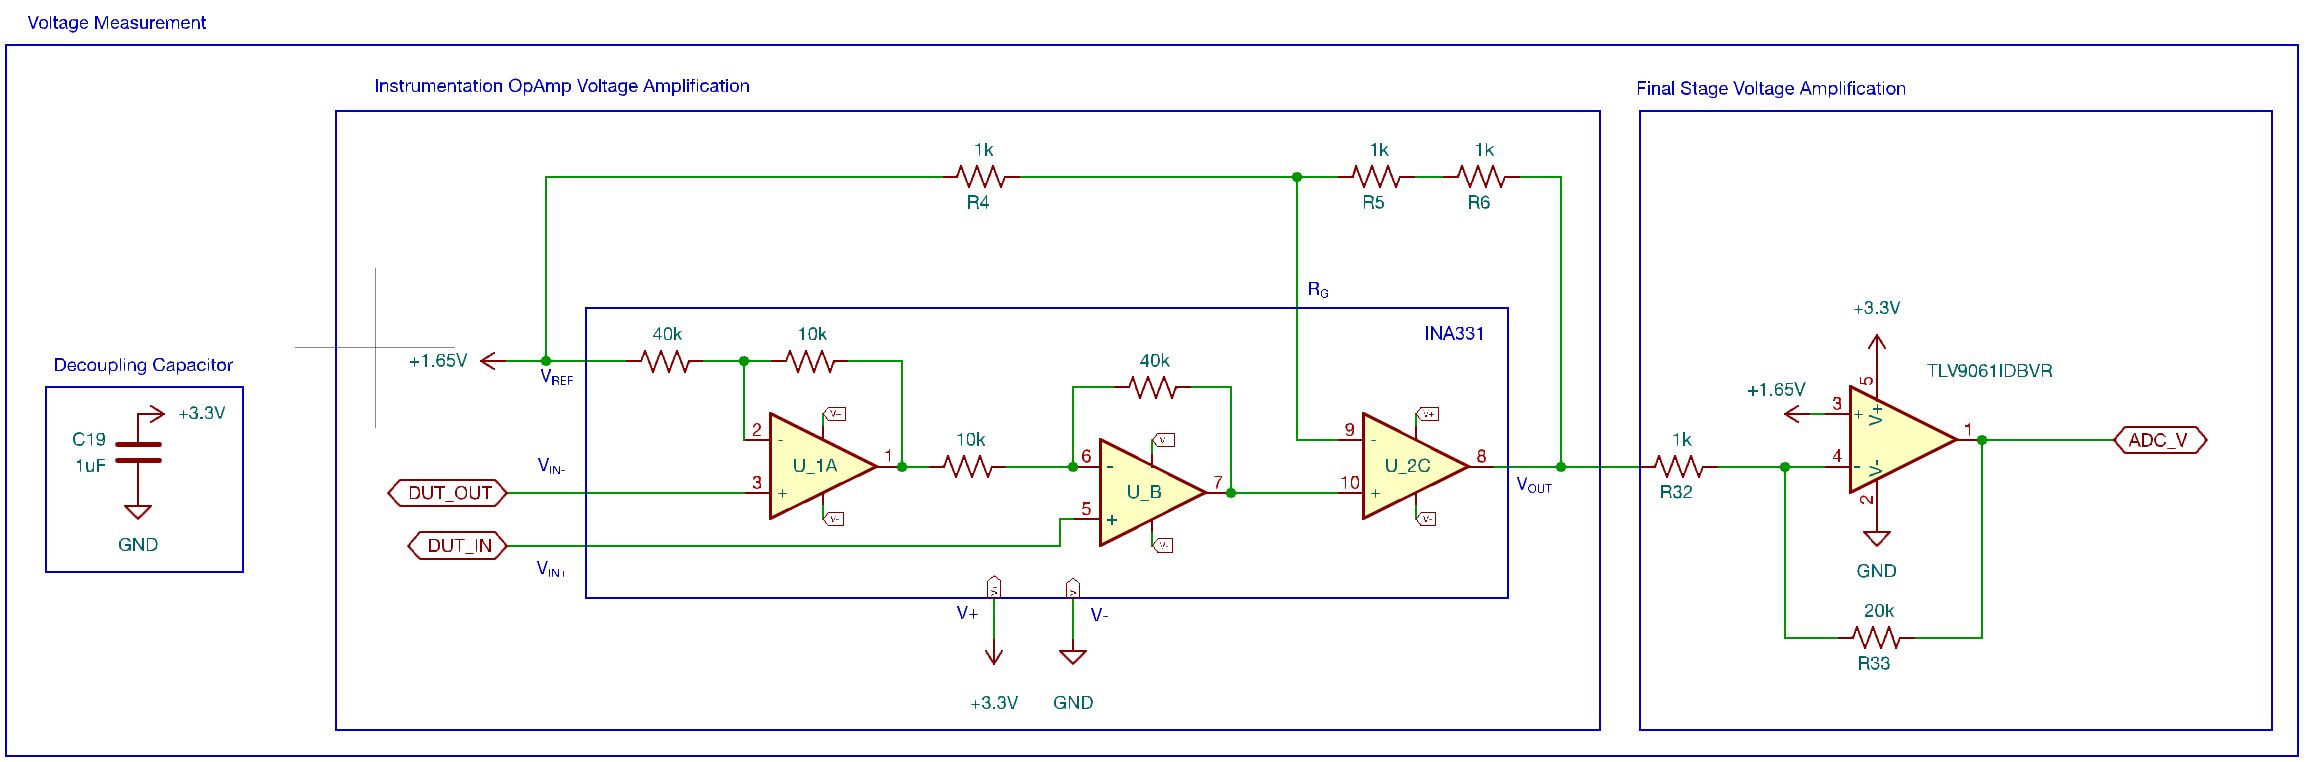
\includegraphics[width=\textwidth]{VMeasSchem.png}
    \caption{Complete Voltage Measurement Stage Circuit}
    \label{fig:vmeas_stage_circuit}
\end{figure}

\subsection{Current Measurement}\label{subsec:design_cur}
The feedback resistor in a \ac{TIA} can be made large without affecting the applied signal to the \ac{DUT}, however it does reduce the bandwidth of the TIA. If $R_{feedback}$ is too large, the TIA will experience significant phase shifts and reduced gain at higher frequencies (referring back to Equation \ref{eq:GBW}). Similarly to the voltage measurement stage, this can be mitigated by using multiple gain stages.

Additionally, biosensing with a fixed voltage perturbation over a wide impedance range means the current can vary from nanoamps (high impedance, low analyte concentration) to milliamps (low impedance, high analyte concentration). To achieve accurate measurement across this dynamic range, a \ac{PGA} is used to amplify the TIA output and ensure that the output voltage remains within the optimal range for the \ac{ADC}. The TIA is also designed with multiple gains by switching the feedback resistor values. This prevents saturation for high currents and maximises resolution for low currents. 

The result is a three-stage current measurement circuit, where the TIA provides the initial current-to-voltage conversion, which is then amplified by a \ac{PGA} before being amplified by a final inverting gain op-amp. The STM32F303K8 also has an internal PGA with an 8MHz GBW and binary gains from $2^1$ - $2^4$. It was unclear whether the added flexibility of a second PGA would outweigh the added noise of an additional gain stage, thus further testing was needed. The PCB was designed with a jumper allowing the internal PGA to be bypassed after testing if needed (see section \ref{sec:PCB}).
